\documentclass[11pt]{article}
\usepackage[margin=1in]{geometry}
\usepackage{graphicx}
\usepackage{booktabs}
\usepackage{amsmath}
\usepackage{xcolor}
\usepackage{float}
\usepackage[hidelinks]{hyperref}
\usepackage{caption}
\captionsetup{font=small,labelfont=bf}
\usepackage{sectsty}
\definecolor{ohno}{HTML}{0072B2}
\definecolor{ssd}{HTML}{D55E00}
\sectionfont{\color{black!80}}
\newcommand{\ohno}{\textcolor{ohno}{\textbf{clustered cis-ohnolog}}}
\newcommand{\ssd}{\textcolor{ssd}{\textbf{clustered SSD-tandem}}}

\title{\textbf{CTCF binding architecture of clustered TF-paralog loci\\
in resting CD4$^+$ T cells:\ ohnolog vs.\ tandem (SSD) clusters}}
\author{Iteration 19 --- Paralogous TF project\\\small ETS P01 genomics platform}
\date{2026-07-18}

\begin{document}
\maketitle

\begin{abstract}
\noindent This report repeats the iteration-19 CTCF analysis in a second, immune-relevant
cell type --- primary \textbf{resting CD4$^+$ $\alpha\beta$ T cells} --- and asks whether the
conclusions drawn from the GM12878 baseline reproduce. Using an ENCODE CD4 T-cell CTCF
ChIP-seq peak set (hg38) over the same clustered-locus windows, we find the same picture:
both \ohno{} and \ssd{} loci are CTCF-enriched over the genome-wide expectation
($\sim$1.5--2.0$\times$ obs/exp) and are \emph{globally indistinguishable} in CTCF density
(Mann--Whitney~U, all $p>0.15$; 0/60 metagene bins at BH-FDR $<0.05$). The one separating
feature is again the \emph{number of CTCF peaks between the two paralog members}
(ohnolog median 3 vs.\ SSD-tandem 0; $p=0.0089$). In CD4 T cells the contrast is sharper than
in GM12878: SSD-tandem pairs frequently carry \emph{no} CTCF peak between their promoters, so
in the 2-member-pair subset the difference persists even after distance normalization
($p=0.021$). As in GM12878, the effect is entangled with the wider inter-member spacing of
ohnolog pairs. The core result --- ohnolog paralogs are separated by more insulator elements
than tandem duplicates --- \textbf{replicates across both cell types}.
\end{abstract}

\section{Data and provenance}
\textbf{CTCF peaks.} ENCODE experiment \texttt{ENCSR470KCE} (TF ChIP-seq, target CTCF,
biosample \emph{Homo sapiens} CD4-positive $\alpha\beta$ T cell, male adult 20 yr ---
primary \emph{resting/unstimulated} CD4 T cell), file \texttt{ENCFF858TLX}
(\emph{IDR-thresholded peaks}, \texttt{bed narrowPeak}, GRCh38, released). Downloaded
2026-07-18. Sanity checks: 40{,}346 peaks; chr1--22, chrX, chrY (male donor).
\emph{Note:} ENCODE has no experiment explicitly labelled ``naive CD4''; this resting
primary CD4 T cell is the closest match (its activated counterpart, \texttt{ENCSR806WWX},
is separate). Genome-wide expected CTCF rate for this set: \textbf{0.0131 peaks/kb}.

\textbf{Locus set.} Identical to the GM12878 analysis: the iteration-16 clustered-locus
catalog (hg38), two clustered classes only, extended $\pm$100~kb. For direct
cross-cell-type comparability the single chrY locus (HSFY1/HSFY2) remains excluded even
though this male sample has chrY signal. Final set: \textbf{47} \ohno{} and \textbf{30}
\ssd{} clusters. Methods (windows, fixed + metagene binning, per-locus metrics, tests) are
exactly as in the GM12878 report; only the CTCF peak file changed.

\section{Results}

\subsection*{Global CTCF density does not separate the two clustered classes}
Over the $\pm$100~kb window both groups sit well above the genome-wide expectation (median
obs/exp $1.96$ ohnolog, $2.05$ SSD-tandem) and none of the global density metrics differ
(Table~\ref{tab:mwu}; all $p>0.15$). The metagene profiles overlap within their bootstrap CI
bands (Fig.~\ref{fig:metagene}) and \textbf{0 of 60} bins reach BH-FDR $<0.05$. Per-flank
enrichment is likewise indistinguishable between groups and shows no left/right asymmetry
within either group (LEFT $p=0.97$, RIGHT $p=0.81$; within-group Wilcoxon $p>0.85$).

\begin{table}[H]
\centering
\small
\caption{Per-locus CTCF metrics in resting CD4 T cells, \ohno{} ($n=47$) vs.\ \ssd{}
($n=30$). Two-sided Mann--Whitney~U; $r_{rb}$ = rank-biserial effect size (negative
$\Rightarrow$ ohnolog $>$ SSD-tandem).}
\label{tab:mwu}
\begin{tabular}{lrrrrr}
\toprule
Metric & median (ohnolog) & median (SSD) & $U$ & $p$ & $r_{rb}$ \\
\midrule
CTCF peaks/kb, window        & 0.0256 & 0.0268 & 718.5 & 0.892 & $-0.019$ \\
CTCF peaks/kb, locus body    & 0.0251 & 0.0105 & 839.0 & 0.159 & $-0.190$ \\
CTCF peaks/kb, flanks        & 0.0250 & 0.0250 & 666.0 & 0.686 & $+0.055$ \\
Observed/expected, window    & 1.962  & 2.052  & 719.0 & 0.888 & $-0.020$ \\
Nearest CTCF to a TSS (bp, min)  & 9445 & 10478 & 707.0 & 0.988 & $-0.003$ \\
Nearest CTCF to TSS (bp, mean)   & 22427 & 22616 & 719.0 & 0.888 & $-0.020$ \\
\textbf{CTCF peaks between members} & \textbf{3.0} & \textbf{0.0} & \textbf{948.5} & \textbf{0.0089} & $\mathbf{-0.345}$ \\
Inter-member TSS distance (bp)   & 74355 & 49409 & 866.0 & 0.094 & $-0.228$ \\
CTCF peaks/kb between members (norm.) & 0.0190 & 0.0000 & 876.0 & 0.067 & $-0.243$ \\
\bottomrule
\end{tabular}
\end{table}

\subsection*{Ohnolog members are separated by more CTCF --- and SSD pairs often by none}
As in GM12878, the distinguishing metric is the count of CTCF peaks between the two paralog
members (ohnolog median 3 vs.\ SSD-tandem 0; $p=0.0089$, $r_{rb}=-0.35$;
Fig.~\ref{fig:between}). The CD4 contrast is stronger at the promoter level: restricting to
2-member pairs, ohnolog pairs have a median of 2 CTCF peaks between their promoters versus
\emph{0} for SSD-tandem pairs ($p=0.010$), and here the per-kb (distance-normalized)
difference is also significant ($0.023$ vs.\ $0.0$ peaks/kb, $p=0.021$;
Fig.~\ref{fig:paired}). Ohnolog promoters are again $\sim$2$\times$ farther apart
(median 52.6~kb vs.\ 25.2~kb, $p=0.15$), so part of the raw-count gap remains a spacing
effect; but the many SSD-tandem pairs with literally zero intervening CTCF indicate that
recent tandem duplicates tend to share a single uninsulated regulatory neighbourhood, whereas
ohnolog paralogs are more often split by an insulator.

\begin{figure}[H]
\centering
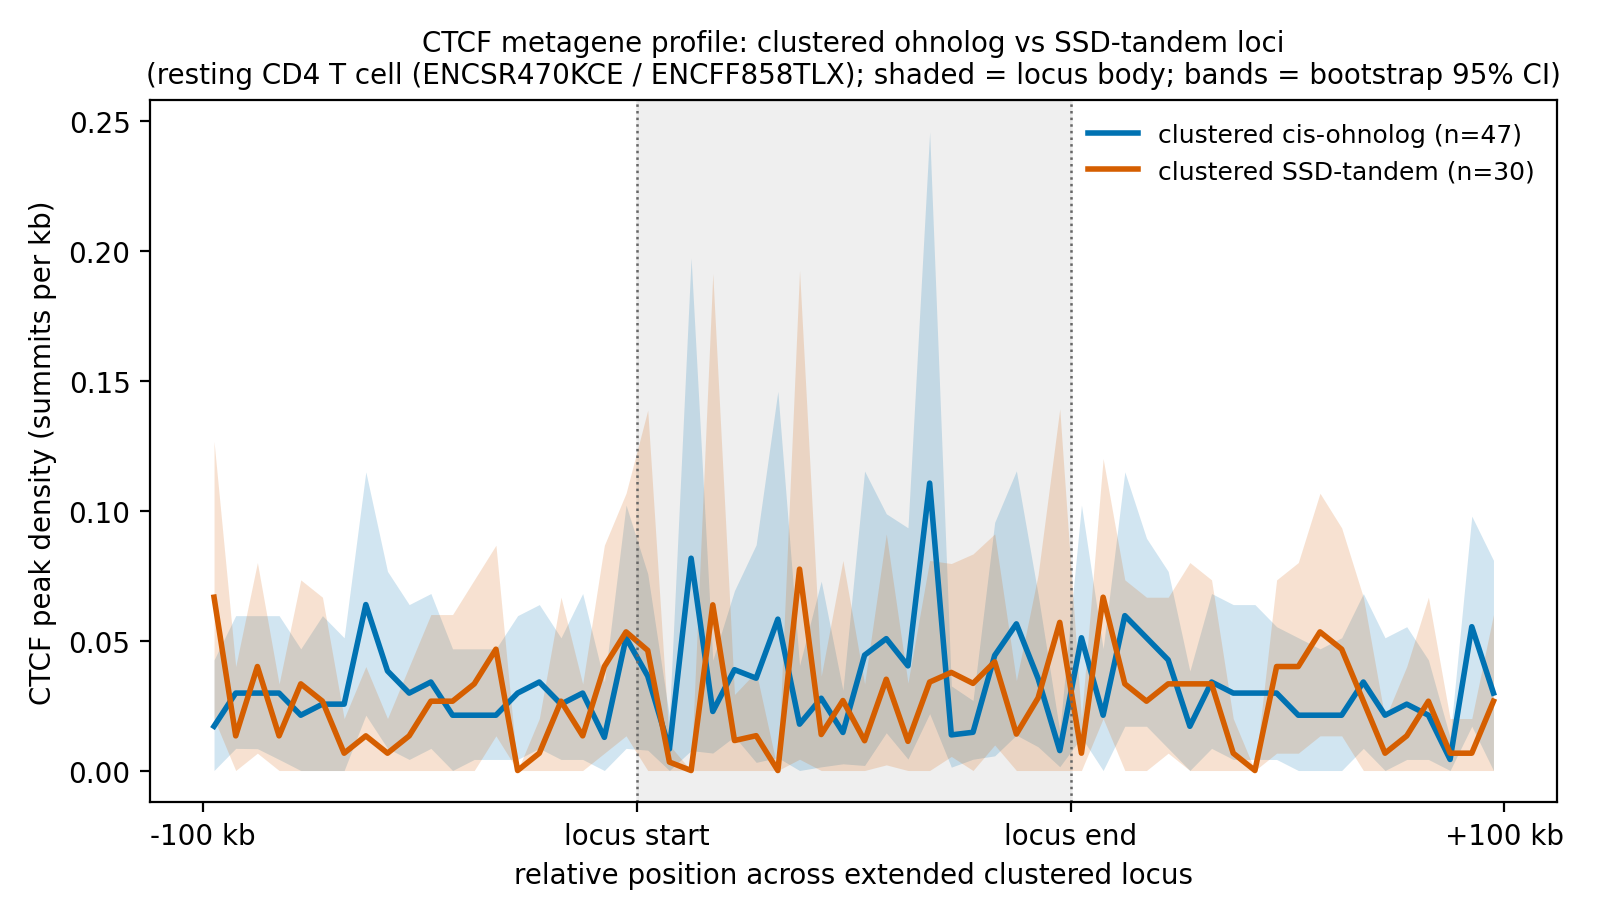
\includegraphics[width=0.9\textwidth]{../results/figures/cd4/ctcf_metagene_clustered_groups.png}
\caption{CD4 T-cell CTCF metagene profile (length-normalized). Lines = mean CTCF summit
density/kb; bands = bootstrap 95\% CI; grey = locus body. The two clustered classes overlap
throughout; no metagene bin survives BH-FDR $<0.05$.}
\label{fig:metagene}
\end{figure}

\begin{figure}[H]
\centering
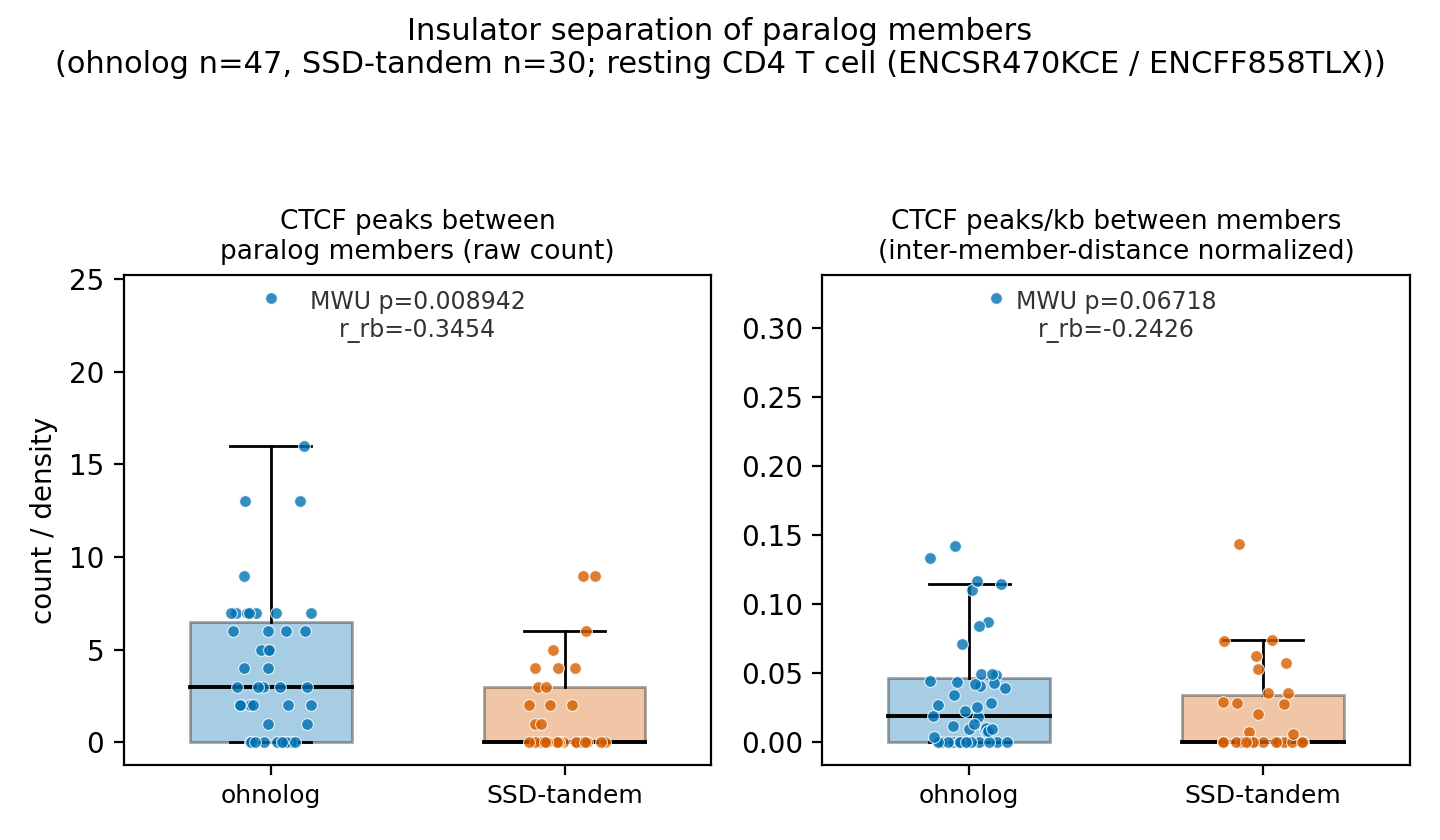
\includegraphics[width=0.72\textwidth]{../results/figures/cd4/ctcf_between_members.png}
\caption{CTCF peaks between paralog members in CD4 T cells. Left: raw count differs
($p=0.0089$). Right: distance-normalized per-kb density (all clustered loci) is borderline
($p=0.067$); in the 2-member-pair subset it reaches significance (Fig.~\ref{fig:paired}).}
\label{fig:between}
\end{figure}

\begin{figure}[H]
\centering
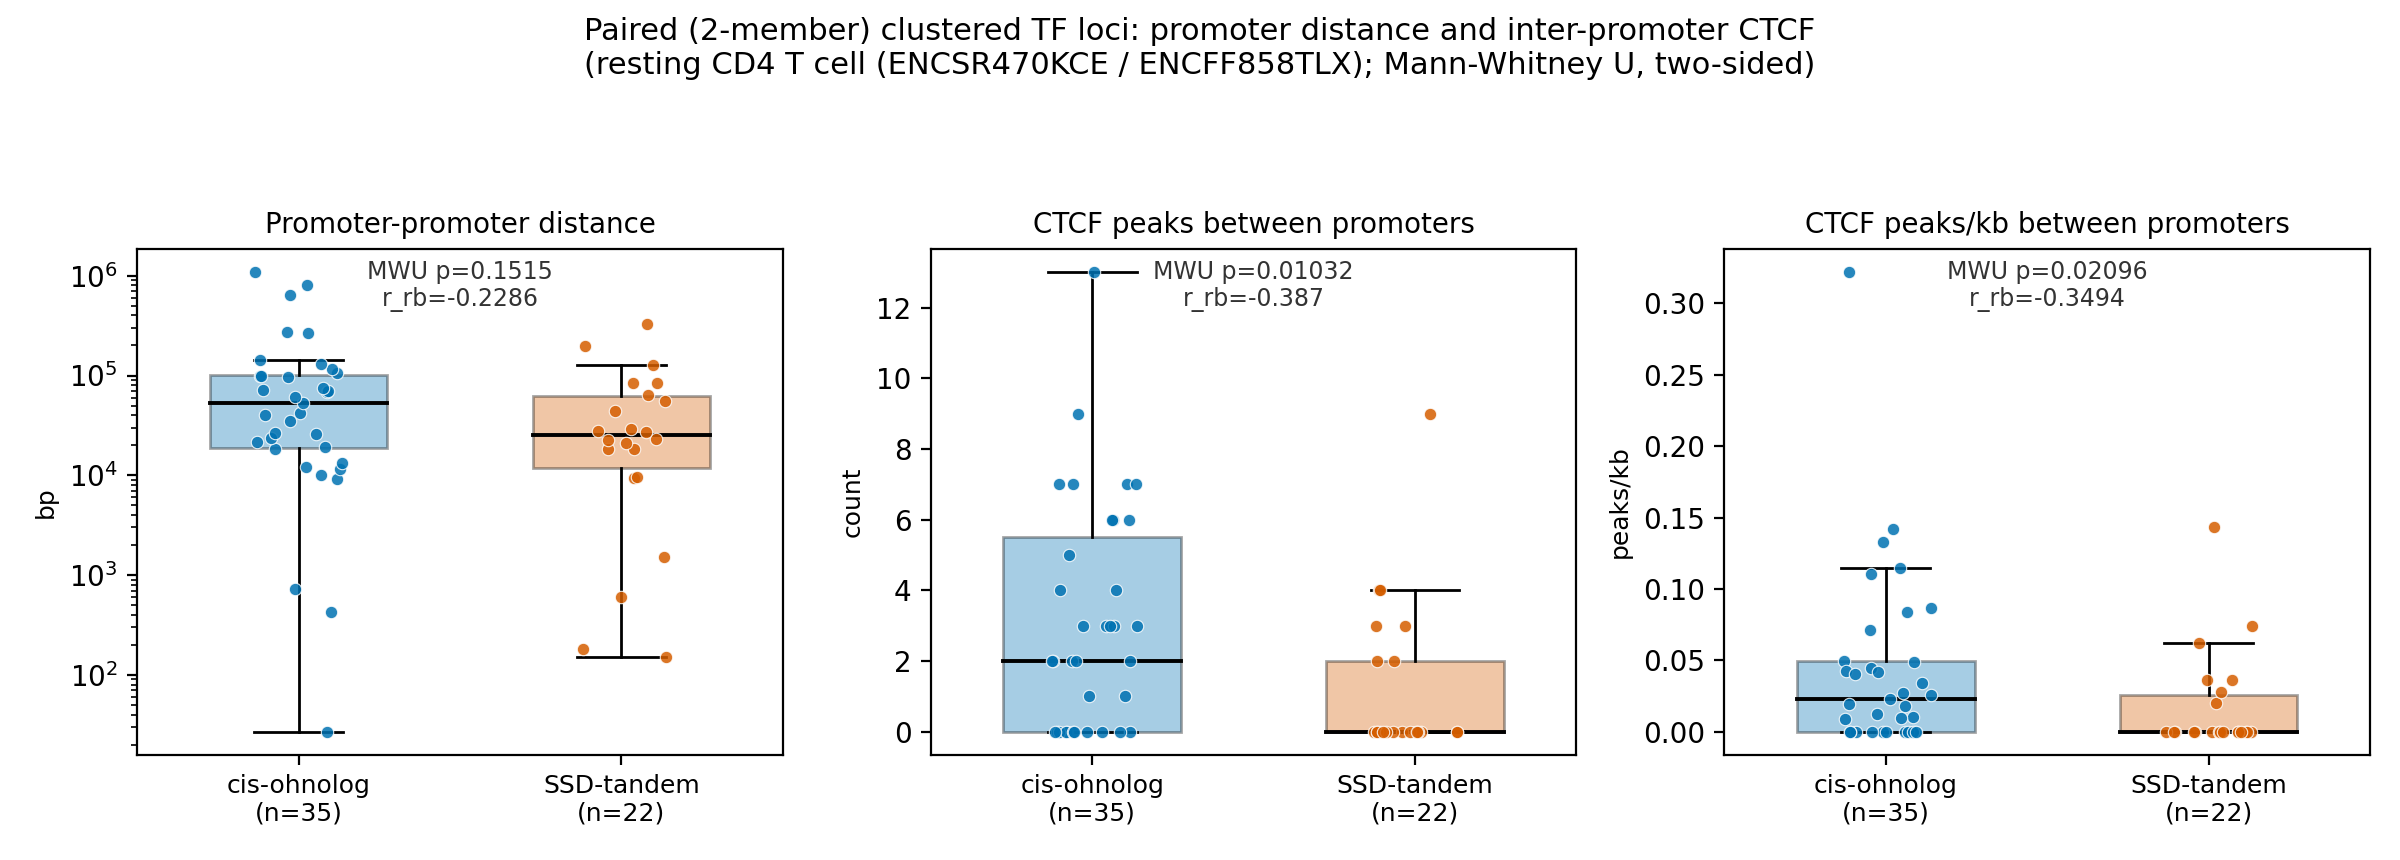
\includegraphics[width=0.98\textwidth]{../results/figures/cd4/paired_promoters_ctcf.png}
\caption{Paired (2-member) clustered loci in CD4 T cells: promoter-promoter distance and
CTCF between promoters. SSD-tandem pairs frequently have zero CTCF between promoters, so both
the raw count ($p=0.010$) and the distance-normalized density ($p=0.021$) differ.}
\label{fig:paired}
\end{figure}

\begin{figure}[H]
\centering
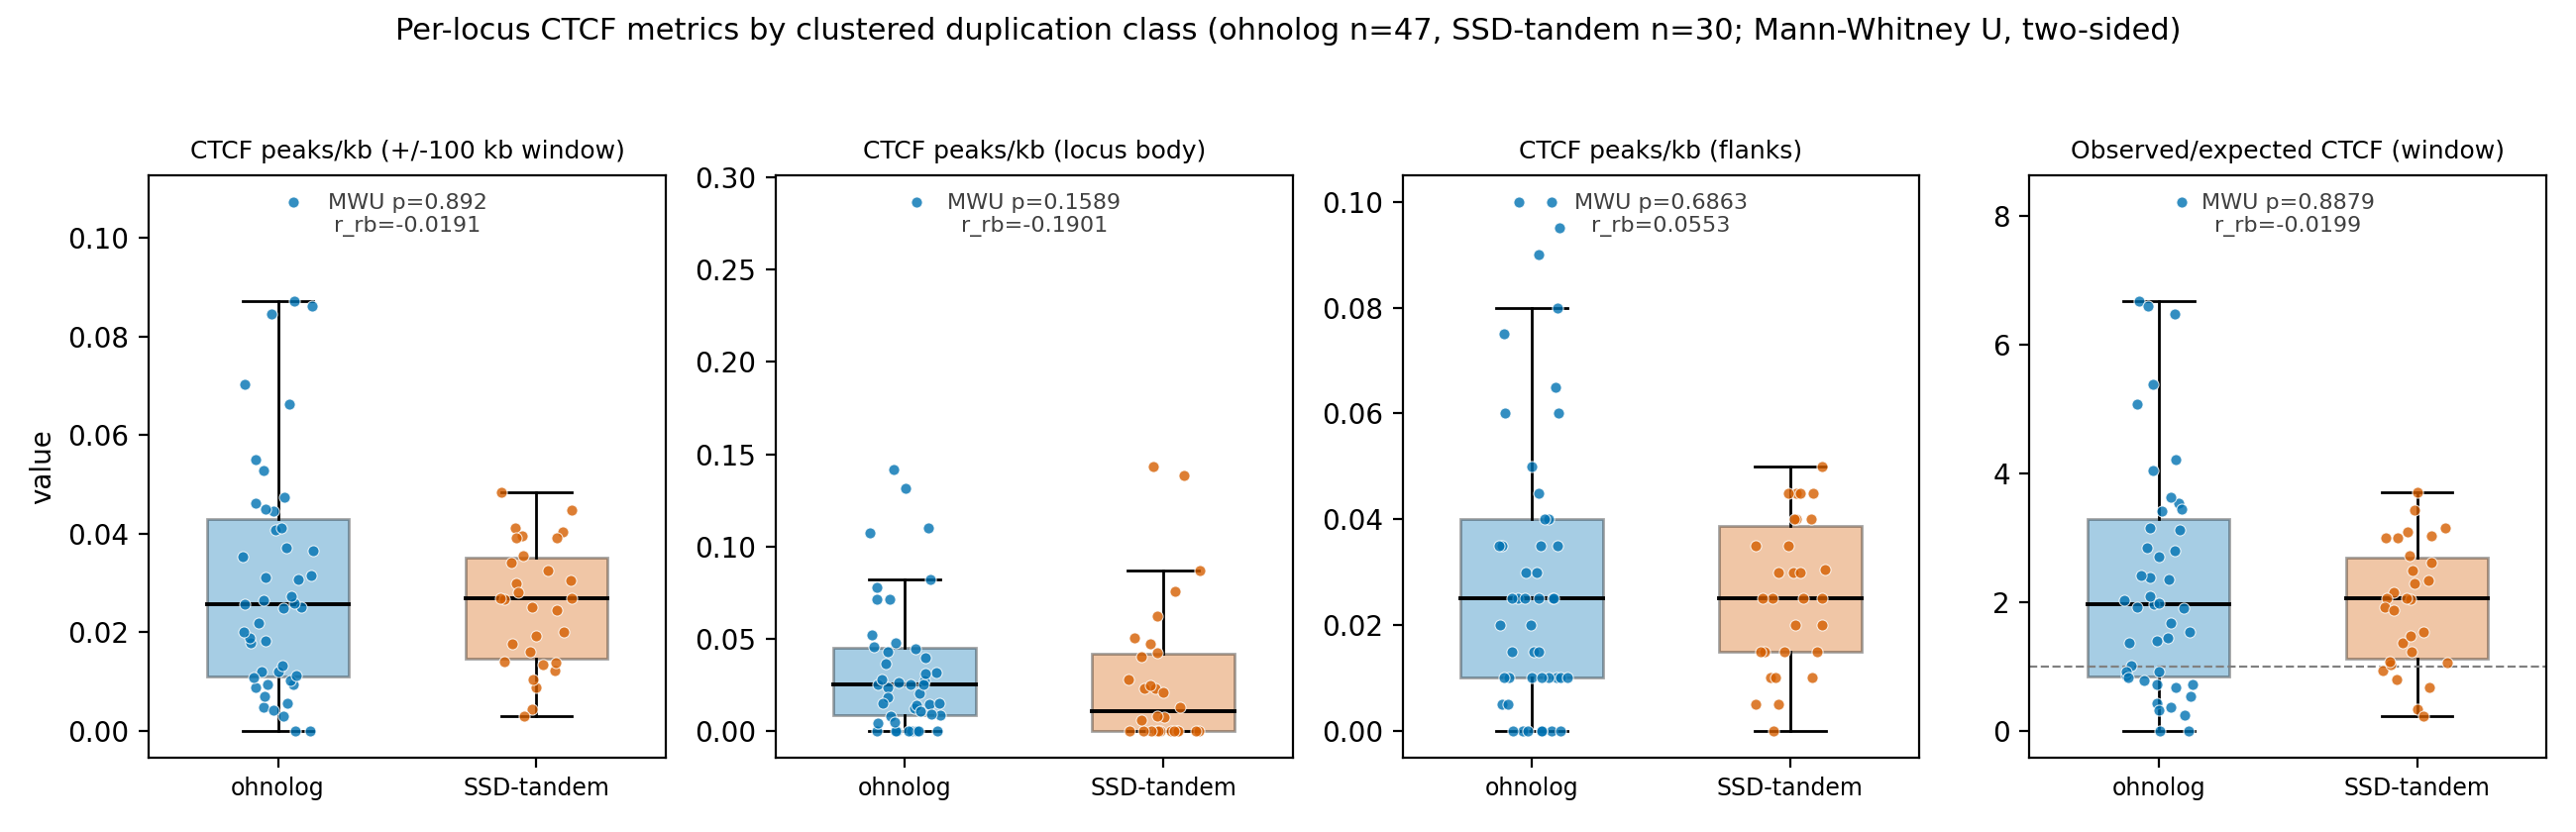
\includegraphics[width=0.95\textwidth]{../results/figures/cd4/ctcf_peaks_per_kb_by_group.png}
\caption{Per-locus global CTCF metrics by class in CD4 T cells; all indistinguishable
between groups, both above the genome-wide expectation.}
\label{fig:box}
\end{figure}

\section{Conclusion --- cross-cell-type reproducibility}
The resting CD4$^+$ T-cell CTCF analysis reproduces every qualitative conclusion of the
GM12878 baseline: (i) both clustered duplication classes occupy CTCF-enriched, statistically
similar overall insulator environments; (ii) the only separating signal is more CTCF peaks
between ohnolog than SSD-tandem paralog members; and (iii) that signal is partly a
consequence of the wider spacing of ohnolog pairs. The one cell-type difference is a matter
of degree, not direction: in CD4 T cells SSD-tandem pairs so often lack any intervening CTCF
that the between-promoter contrast survives distance normalization in the pair subset,
whereas in GM12878 it did not. That the finding holds in two independent cell types --- an
EBV B-lymphoblastoid line and primary resting CD4 T cells --- argues it reflects a
constitutive, mechanism-linked feature of the loci rather than a cell-line artefact.

\paragraph{Caveats.} (i)~Two cell types now, but still a limited panel; CTCF is largely
constitutive. (ii)~Small groups (47 vs.\ 30 clusters) --- per-locus tests are underpowered
and the inter-member-distance confounder ($p=0.09$) is not resolved. (iii)~Fixed-bp and
metagene binnings are reported separately. (iv)~The chrY locus was excluded for
cross-cell-type comparability; ``LEFT/RIGHT'' flanks are genomic, not strand-oriented.
(v)~ENCODE has no explicitly ``naive'' CD4 CTCF experiment --- the resting primary CD4 T cell
(\texttt{ENCSR470KCE}) is used as the closest available proxy.

\end{document}
